% statistics_and_probability:x20 GDC:YES
\begin{question}
  \hspace*{\fill} [Note maximale: 12]\par
  \medskip
  \noindent Il y a 50 boîtes dans une usine. Les poids, w en kg, sont divisés en 5 classes, comme le montre le tableau ci-dessous.\par
  \medskip
  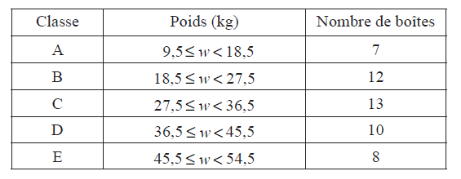
\includegraphics[scale=0.5]{tableau_poids_boite}\par
  \medskip
  (a) Montrez que le poids moyen estimé des boîtes est 32 kg.\hspace*{\fill} [3]\par
  \medskip

  (b) Dans l’usine, il y a x boîtes marquées « Fragile ». Elles sont toutes dans la\par
  \hspace{2em}classe E. Le poids moyen estimé de toutes les autres boîtes dans l’usine est 30 kg.\par
  \hspace{2em}Calculez la valeur de x.\hspace*{\fill} [4]\par
  \medskip

  (c) Une livraison de y boîtes supplémentaires, toutes ayant un poids dans la\par
  \hspace{2em}classe D, est apportée à l’usine. Le poids moyen estimé total de toutes les boîtes\par
  \hspace{2em}dans l’usine est inférieur à 33 kg . Trouvez la plus grande valeur possible de y.\hspace*{\fill} [5]\par

\end{question}

